\RequirePackage{plautopatch}
\documentclass[uplatex,dvipdfmx,10pt,a4paper,notitlepage,oneside,twocolumn]{abst_jsarticle}
% notitlepage : \titlepage は独立しない
% oneside : 奇数・偶数ページは同じデザイン
% twocolumn : 2段組
% \setlength{\textwidth}{\fullwidth}
% 本文領域はページ一杯で, 傍注の幅を取らない
\usepackage[dvipdfmx]{graphicx}
\usepackage[dvipdfmx,x11names]{xcolor}
\usepackage{amsmath,amssymb}
% \numberwithin{equation}{section}
\usepackage{url}
\usepackage{bm}
\usepackage[hang, small, bf, labelsep=quad]{caption}

\columnsep=10mm
\setlength{\hoffset}{-0.85cm}
\setlength{\voffset}{-2.0cm}
\setlength{\textwidth}{53zw}   %横25字
\setlength{\textheight}{78zw}

% \renewcommand{\baselinestretch}{0.8}
%upTex(ptex2pdf)
\usepackage{fancyhdr}
\fancypagestyle{firstpage}
{
   \fancyhead[L]{中央大学大学院理工学研究科2024年度修士論文}
   \fancyhead[R]{}
   \fancyfoot{}
   \renewcommand{\headrulewidth}{0pt}
}

\title{
\textbf{\textgt{煙シミュレーションのための部分空間法の高速化}}\\
%\vspace*{0.3cm}
\textsf{Accelerated Subspace Method for 3D Smoke Simulation}\\
}
\author{
{\large \textbf{\textgt{情報工学専攻 須之内 俊樹}}}\\
{\large \textsf{Toshiki SUNOUCHI}}
}

\date{}
\pagestyle{empty}

\begin{document}

\maketitle
%%%%%%%%%%%%%%%%%%%%%%%%%%%%%%
\thispagestyle{firstpage}

\begin{abstract}
本研究では部分空間法の前処理に対して,計算時間を高速化する手法を提案する.部分空間法を適用することで,シミュレーションは大幅に高速化することができるが,前処理に膨大な計算時間がかかることが課題である.そこで本研究は,前処理をシミュレーション時間に対して分割し,前処理全体の計算時間を削減する手法を提案する.計算機実験の結果,前処理のボトルネックとなっている基底計算のための特異値分解の高速化を確認し,前処理の高速化に有効であると示すことができた.
\end{abstract}


\vspace{1zw} \noindent
\textbf{\textgt{キーワード:}} 
流体シミュレーション,部分空間法,スナップショット固有直交分解,立体求積法.


\section{はじめに} \label{sec:section1}

流体シミュレーションは,工学およびコンピュータグラフィックスの分野において広く利用されている.コンピュータグラフィックスの分野では,現実的な水や煙のアニメーションを生成し,映像作品やゲームの演出に活用されている.コンピュータグラフィックスにおいては,物理的に厳密なシミュレーションよりも,視覚的に自然な動きを高速に計算することが求められる.

近年,より高解像度の流体シミュレーションが求められる中で,計算負荷の増大が課題となっている.そのため,高速化手法の研究が活発に進められており,特に大規模並列計算技術の適用が重要視されている.多くの高速化手法がGPU上での実装を前提として検討されている.

計算負荷の削減手法の一つとして,前処理によりシミュレーション計算に使用する行列の次元を削減する部分空間法が存在する.部分空間法を適用することで,シミュレーション計算そのものは高速化されるが,前処理に要する計算負荷やメモリ使用量が大きくなるという課題がある.
本研究では,部分空間法の計算負荷を削減することにより,前処理に要する時間の短縮を図ることを目的とする.

\section{関連研究}
\subsection{煙の流体シミュレーション}
下記の式\ref{eq:Navie}で表される式を,ナビエ・ストークス方程式とよび,これは流体力学の支配方程式である.非線形二階微分方程式となっており,代数的に一般解を求める事ができない.
式\ref{eq:uncompressed} は流体の非圧縮性条件であり,煙のシミュレーションにおいて流速が著しく大きい場合を除き,利用することが可能である.
	\begin{equation}\label{eq:Navie}
		\frac{\partial}{\partial t}\bm{u} (t)  = - (\bm{u} (t)  \boldsymbol{\cdot}\nabla) \bm{u} (t)   - \frac{1}{\rho}\nabla \bm{p} (t)  + \nu\nabla^2\bm{u} (t)  + \bm{f}
	\end{equation}
	
	\begin{equation}\label{eq:uncompressed}
		\nabla\boldsymbol{\cdot}\bm{u} (t)  = 0
	\end{equation}
	
ナビエ・ストークス方程式の数値解法の中でも, \cite{MAC,Chorin}において全ての項を個別に分割して解く手法としてフラクショナルステップ法が提案されている.フラクショナルステップ法の分割において,式 \ref{eq:Navie} の右辺の第一項を移流項,第二項を圧力項,第三項を粘性項,第四項を外力項と呼ぶ.\cite{Chorin}のフラクショナルステップ法は,中間子$\bm{u_0}$から$\bm{u_3}$を用いて,ナビエ・ストークス方程式を以下のように分割する.
\[
	\bm{u_0} =  \bm{u} (t)  - \varDelta t \bm{f} 	
\]
\[
	\bm{u_1}(\bm{x}) = \bm{u_0}(\bm{x}  - \varDelta t \bm{u_0})
\]
\[
	\bm{u_2}   =  \bm{V}\bm{u_1}
\]
\[
	\bm{b} = \bm{W}\bm{u_2}
\]
\[
	\bm{p} = \bm{A^{-1}}\bm{b}
\]
\[
	\bm{u_3}  =  \bm{u_2} - \bm{Y}\bm{p} 
\]
\subsection{部分空間法}
 	\[
 		\bm{\tilde{x}}  = \bm{A^T}\bm{x}
 	\]
	\[
		\bm{x} = \bm{A}\bm{\tilde{x}} 
	\]	
	また,$\bm{\tilde{x'}}  = \bm{A^T}\bm{x'}$を満たす$n$次元ベクトル$\bm{x'}$,$r$次元ベクトル$\bm{\tilde{x'}} $について,以下の2式が成り立つような,任意の$m \times n$行列$\bm{F}$,任意の$m \times r$行列$\bm{\tilde{F}}$を考える.
	\[
		\bm{x'} = \bm{F}\bm{x}
	\]
	\[
		\bm{\tilde{x'}}  = \bm{\tilde{F}}\bm{\tilde{x}} 
	\]
$\bm{\tilde{x'}}  = \bm{A^T}\bm{x'}$に,$\bm{x'} = \bm{F}\bm{x}$と,$\bm{x} = \bm{A}\bm{\tilde{x}} $を代入することで,
	\[
		\bm{\tilde{x'}}  = (\bm{A^T}\bm{F}\bm{A})\bm{\tilde{x}} 
	\]
	が得られる.$\bm{\tilde{x'}}  = \bm{\tilde{F}}\bm{\tilde{x}} $と比較すると,
	\[
	\bm{\tilde{F}} = \bm{A^T}\bm{F}\bm{A}
	\]
	が得られる.
\section{スナップショット分割による高速化}

\subsection{フラクショナルステップ法への部分空間法の適用}
\begin{align*}
 \bm{U_2^T}\bm{u_2}	& = (\bm{U_2^T}\bm{V}\bm{U_1})\bm{U_1^T}\bm{u_1} 					&\bm{\tilde{u_2}} 		&= \bm{\tilde{V}}\bm{\tilde{u_1}}	\\
 \bm{P^T}\bm{b}		& = (\bm{P^T}\bm{W}\bm{U_2})\bm{U_2^T}\bm{u_2}        				&\bm{\tilde{b}}			&= \bm{\tilde{W}}\bm{\tilde{u_2}}	\\
 \bm{P^T}\bm{p} 		&= (\bm{P^T}\bm{A}^{-1}\bm{P})\bm{P^T}\bm{b}						&\bm{\tilde{p}}			&= \bm{\tilde{A}}\bm{\tilde{b}}\\
 \bm{U_3^T}\bm{u_3} 	&=  \bm{U_2^T}\bm{u_2} - (\bm{U_3^T}\bm{Y}\bm{P})\bm{P^T}\bm{p}	&\bm{\tilde{u_3}}		&= \bm{\tilde{u_2}}  -  \bm{\tilde{Y}}\bm{\tilde{p}}
\end{align*}

\subsection{部分空間法の高速化手法の提案}
部分空間法の前処理において,基底の計算と行列の射影の計算量はスナップショットの$2$乗に比例し,前処理の大多数の時間を占めている.本節では部分空間法の前処理の高速化を達成するため,スナップショットを$d$個に分割する手法を提案する.

部分空間法の基底の計算に用いるスナップショットを$d$分割することによって,基底1つの計算負荷$O(nm^2)$が$\frac{1}{d^2}$に削減される.アルゴリズム全体では$d$回計算するため,計算負荷は$\frac{1}{d}$になることが期待できる.行列の射影計算も分割した基底ごとに行う.空間計算量のボトルネックは分割前のスナップショット行列であり,分割前と変わらない.しかし,特異値分解する行列のサイズが$\frac{1}{d}$になることで,GPUを用いた大規模高速計算と併用する場合,GPUメモリの削減が期待できる.空間計算量をGPUが一度に扱うことができる値まで削減することで,並列計算による高速化が期待できる一方で,特異値分解の回数が$d$倍になることで,CPU-GPU間のデータ通信の時間が増加することに注意が必要である.

\section{計算機実験}
本研究では,c++と線形代数ライブラリEigenを用いて,文献\cite{fedkiw}の煙の流体シミュレーションを行うソフトウェアを実装した.立方体形状のシミュレーション空間の底面中心から,煙が立ち上る様子をシミュレーションし,そのデータを元に部分空間法による次元削減を行なった.また,OpenGLを用いてスライスベースのボリュームレンダリングを行い,実験結果を可視化するソフトウェアを実装した.これによって得られたシミュレーション結果と,提案手法の計算負荷と削減後のデータの精度について調査を行った.計算負荷の評価は,部分空間法の基底を計算する前処理と行列の射影について実行時間を計測した.データの精度は非線形項の部分空間への射影手法\cite{projection_base}を参考に,L2誤差を用いて評価を行なった.ここでL2誤差は次元削減前後のベクトル$\bm{u}$と$\bm{\tilde{u}}$について,以下のように表される.

\[
L_2 = \frac{|| \bm{u} - \bm{\tilde{u}} ||_2}{||  \bm{u} ||_2}
\]

\begin {table}[htbp]
    \centering
  \caption{基底計算における解像度と分割数ごとの実行時間(秒)}
  \label{tab:basis}
  \begin {tabular}{rrrrr} \hline
    \multicolumn{1}{c}{解像度} 					&\multicolumn{1}{c}{分割なし} 		&\multicolumn{1}{c}{分割数2}			&\multicolumn{1}{c}{分割数4} 		&\multicolumn{1}{c}{分割数10}\\ \hline
    $64^3$ 					& 23.428 			&14.564	 		&8.981	 	&3.780\\
    $128^3$ 				& 190.541 		&118.489 			& 69.615 		&33.427\\ \hline
  \end {tabular}
\end {table}

\begin {table}[htbp]
    \centering
  \caption{行列の射影における解像度と分割数ごとの実行時間(秒)}
  \label{tab:projection}
  \begin {tabular}{rrrrr} \hline
    \multicolumn{1}{c}{解像度} 					&\multicolumn{1}{c}{分割なし} 		&\multicolumn{1}{c}{分割数2}			&\multicolumn{1}{c}{分割数4} 		&\multicolumn{1}{c}{分割数10}\\ \hline
    $64^3$ 					& 3.514 			&2.823	 		&0.846	 		&0.666\\
    $128^3$ 				& 5.206 			& 3.061 			& 3.050 		&3.975\\ \hline
  \end {tabular}
\end {table}

\begin{figure}[htbp]
\centering
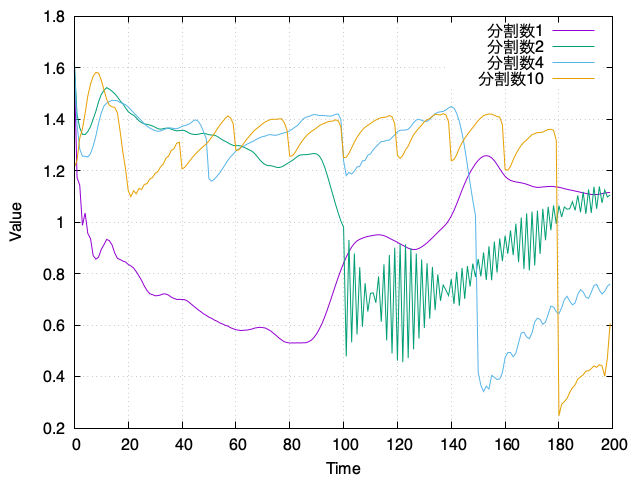
\includegraphics[width=80mm]{images/64error.png}
\caption{$解像度64^3におけるL_2誤差$}
\label{fig:64error}
\end{figure}

\begin{figure}[htbp]
\centering
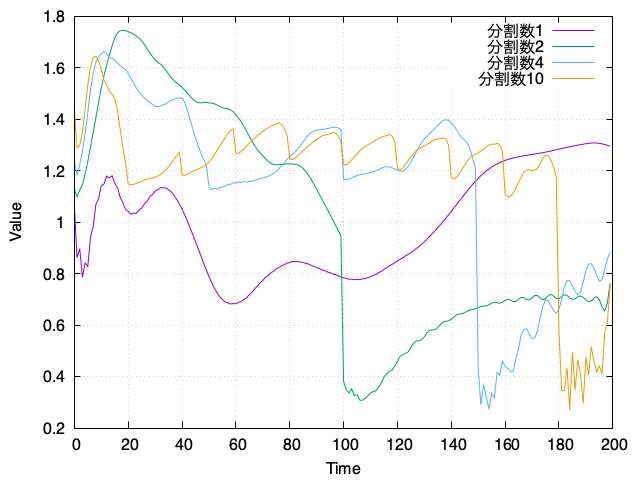
\includegraphics[width=80mm]{images/128error.png}
\caption{$解像度128^3におけるL_2誤差$}
\label{fig:128error}
\end{figure}

\section{考察}

\section{終わりに}
流体シミュレーションにおける部分空間法の前処理にかかる計算時間に対し,スナップショットを分割することによって高速化する手法を提案した.特に基底計算については分割数に応じた高速化を達成し,前処理全体の高速化を達成した.スナップショット分割によるシミュレーションの結果に関して,$L_2$誤差では差が認められたものの,見た目の上では問題ない範囲であった.
% 参考文献
\begin{thebibliography}{99}

\bibitem{Chorin}
A. J. Chorin. Numerical Solution of the Navier-Stokes Equations. \textit{Mathematics of Computation}, 22(104): 745--762, 1968.

\bibitem{fedkiw}
R. Fedkiew, J. stam, H. Jensen. Visual simulation of smoke. In \textit{Proceedings of SIGGRAPH 01}, 15--22, 2001.

\bibitem{stam}
J. Stam. Stable Fluids. In \textit{SIGGRAPH 99 Conference Proceedings, Annual Conference Series}, pages 121--128, 1999.

\bibitem{projection_base}
A. Treuille, A. Lewis, and Z. Popovic. Model Reduction for Real-time Fluids. \textit{ACM Transactions on Graphics},25(3):826--834, 2006.

\bibitem{subspace}
T. Kim, J. Delaney. Subspace Fluid Re-Simulation. \textit{ACM Transactions on Graphics},32(4): 62:1--62:9, 2013.

\end{thebibliography}
\end{document}
